\chapter{Results}
In this chapter, the proposed algorithm is evaluated on the LPW data set, and numerical results are presented, followed by a discussion of the results and possible improvements.
\section{Evaluation}
The evaluation of the proposed algorithm is done by calculating the error of the pupil center. The data set labels the center of the ellipse, not the actual ellipse parameter. Therefore, the evaluation of the actual fit of the ellipse was conducted manually, and no numerical results for the fit are presented. For the evaluation of the pupil center, the ground truth notation explained in subsection \ref{subsec:ground_truth} is used. The error is calculated in the x and y direction separately, and a KDE Plot is used to display the error density of the estimation. The error is calculated for each frame, totaling 2000 frames per video. The standard deviation is calculated and drawn into the KDE plot as an ellipse, giving insight into the algorithm's accuracy. The noise changes throughout the video because of eye movement and blinking. As mentioned in the introduction, the algorithm cannot detect if the eye is open or closed. Therefore, a significant error deviation is possible and filtered out if it is more significant than three times the standard deviation of the complete video. To filter the error, the z score is introduced. The z score is a statistical measure that tells how far a point is from the mean of a data set in terms of standard deviations. All errors with a z score greater than three are declared outliers for the evaluation. 

\section{Discussion}
The algorithm's performance can be split up into Accuracy, Speed, Robustness and Noise. The error of the pupil center measures the accuracy. The algorithm's speed is given in frames per second and is calculated with the mean of the total time taken for processing 2000 frames. The robustness is measured by the number of outliers the algorithm produces. The noise is hard to evaluate because the data set is very diverse and eye movement during the video changes the amount of noise present.
\subsection{Accuracy}
The algorithm's accuracy can be seen in the KDE plot of an example video. The KDE plot is shown in figure \ref{fig:kde} and shows the error density of the pupil center estimation. 

\begin{figure}[h]
        \centering
        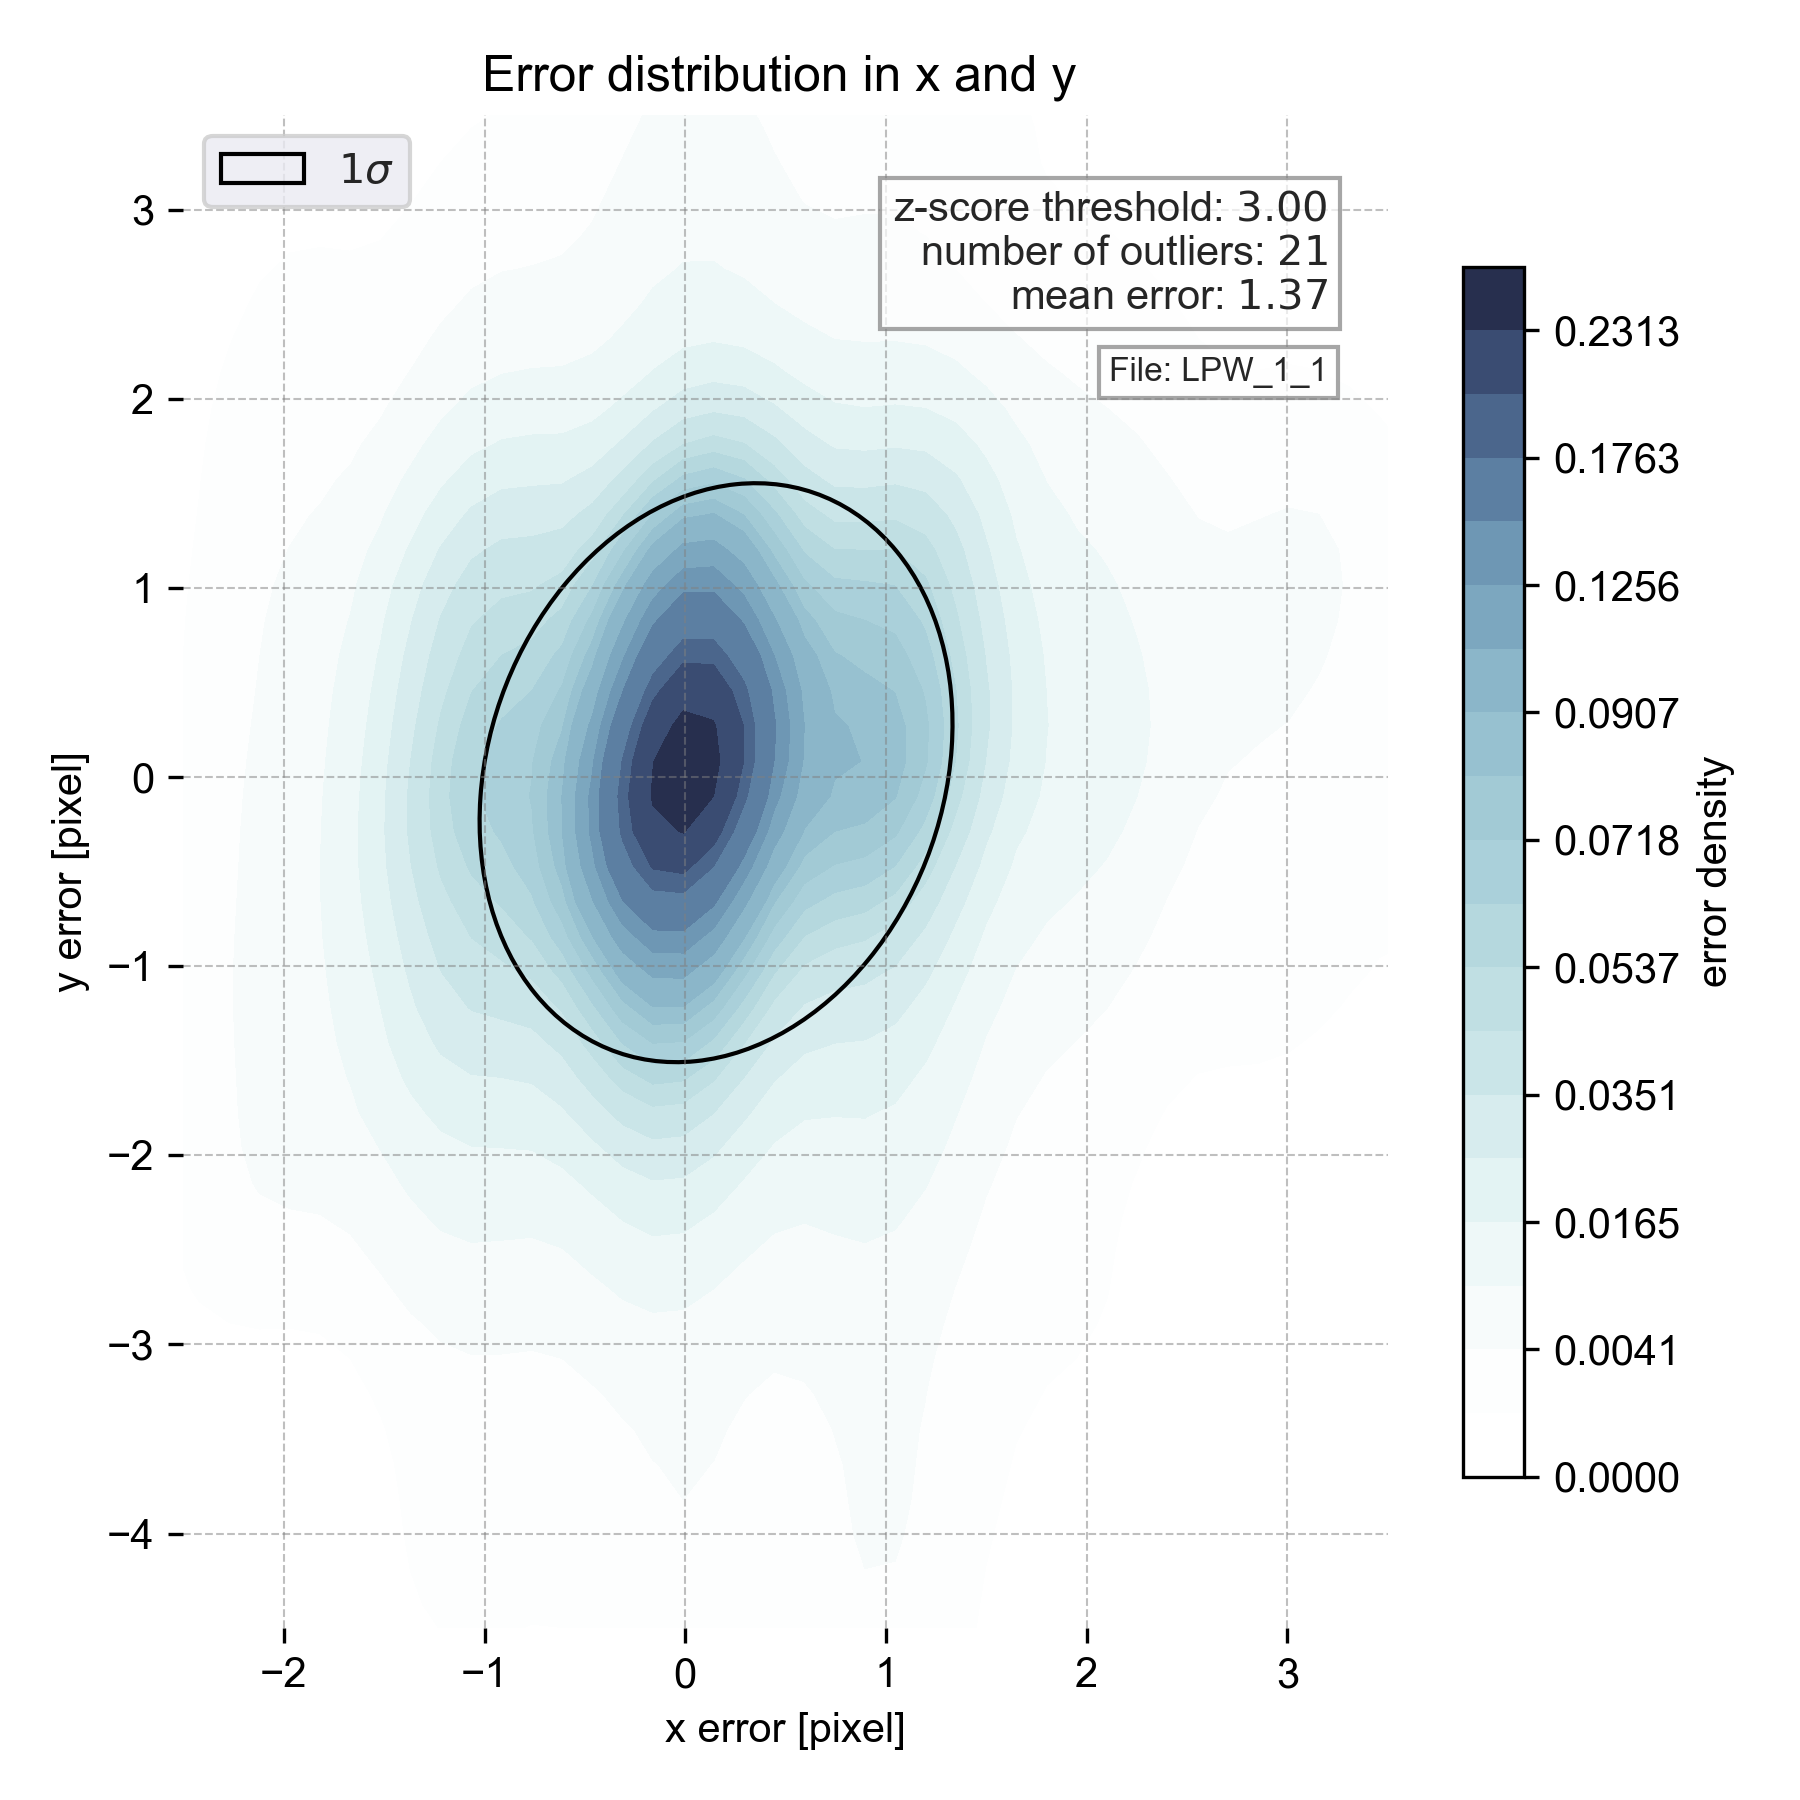
\includegraphics[width=\textwidth]{plots/LPW_1_1pre.png}
    \caption{Error KDE plot of the pupil center estimation}
    \label{fig:kde}
\end{figure}
Here, the standard deviation in the y direction is bigger than in the x direction. The reason for the difference in the axes has to do with the experimental setup of the LPW data set. Because in most of the videos, the light source is reflected in the pupil when the participant is looking to the left, leaving only a small portion of pupil contour on the right side of the pupil. Because the contour information is not complete and more information on the y-axis is missing. Therefore the y-axis probability error fluctuates more than the x-axis. The same observation persists and increases when using different scaling of the video. Here is a comparison between the full-size video (640x480) with the scaling of 0.5 (320x240) 
\begin{figure}[h]
    \centering
    \begin{subfigure}{0.49\textwidth}
        \centering
        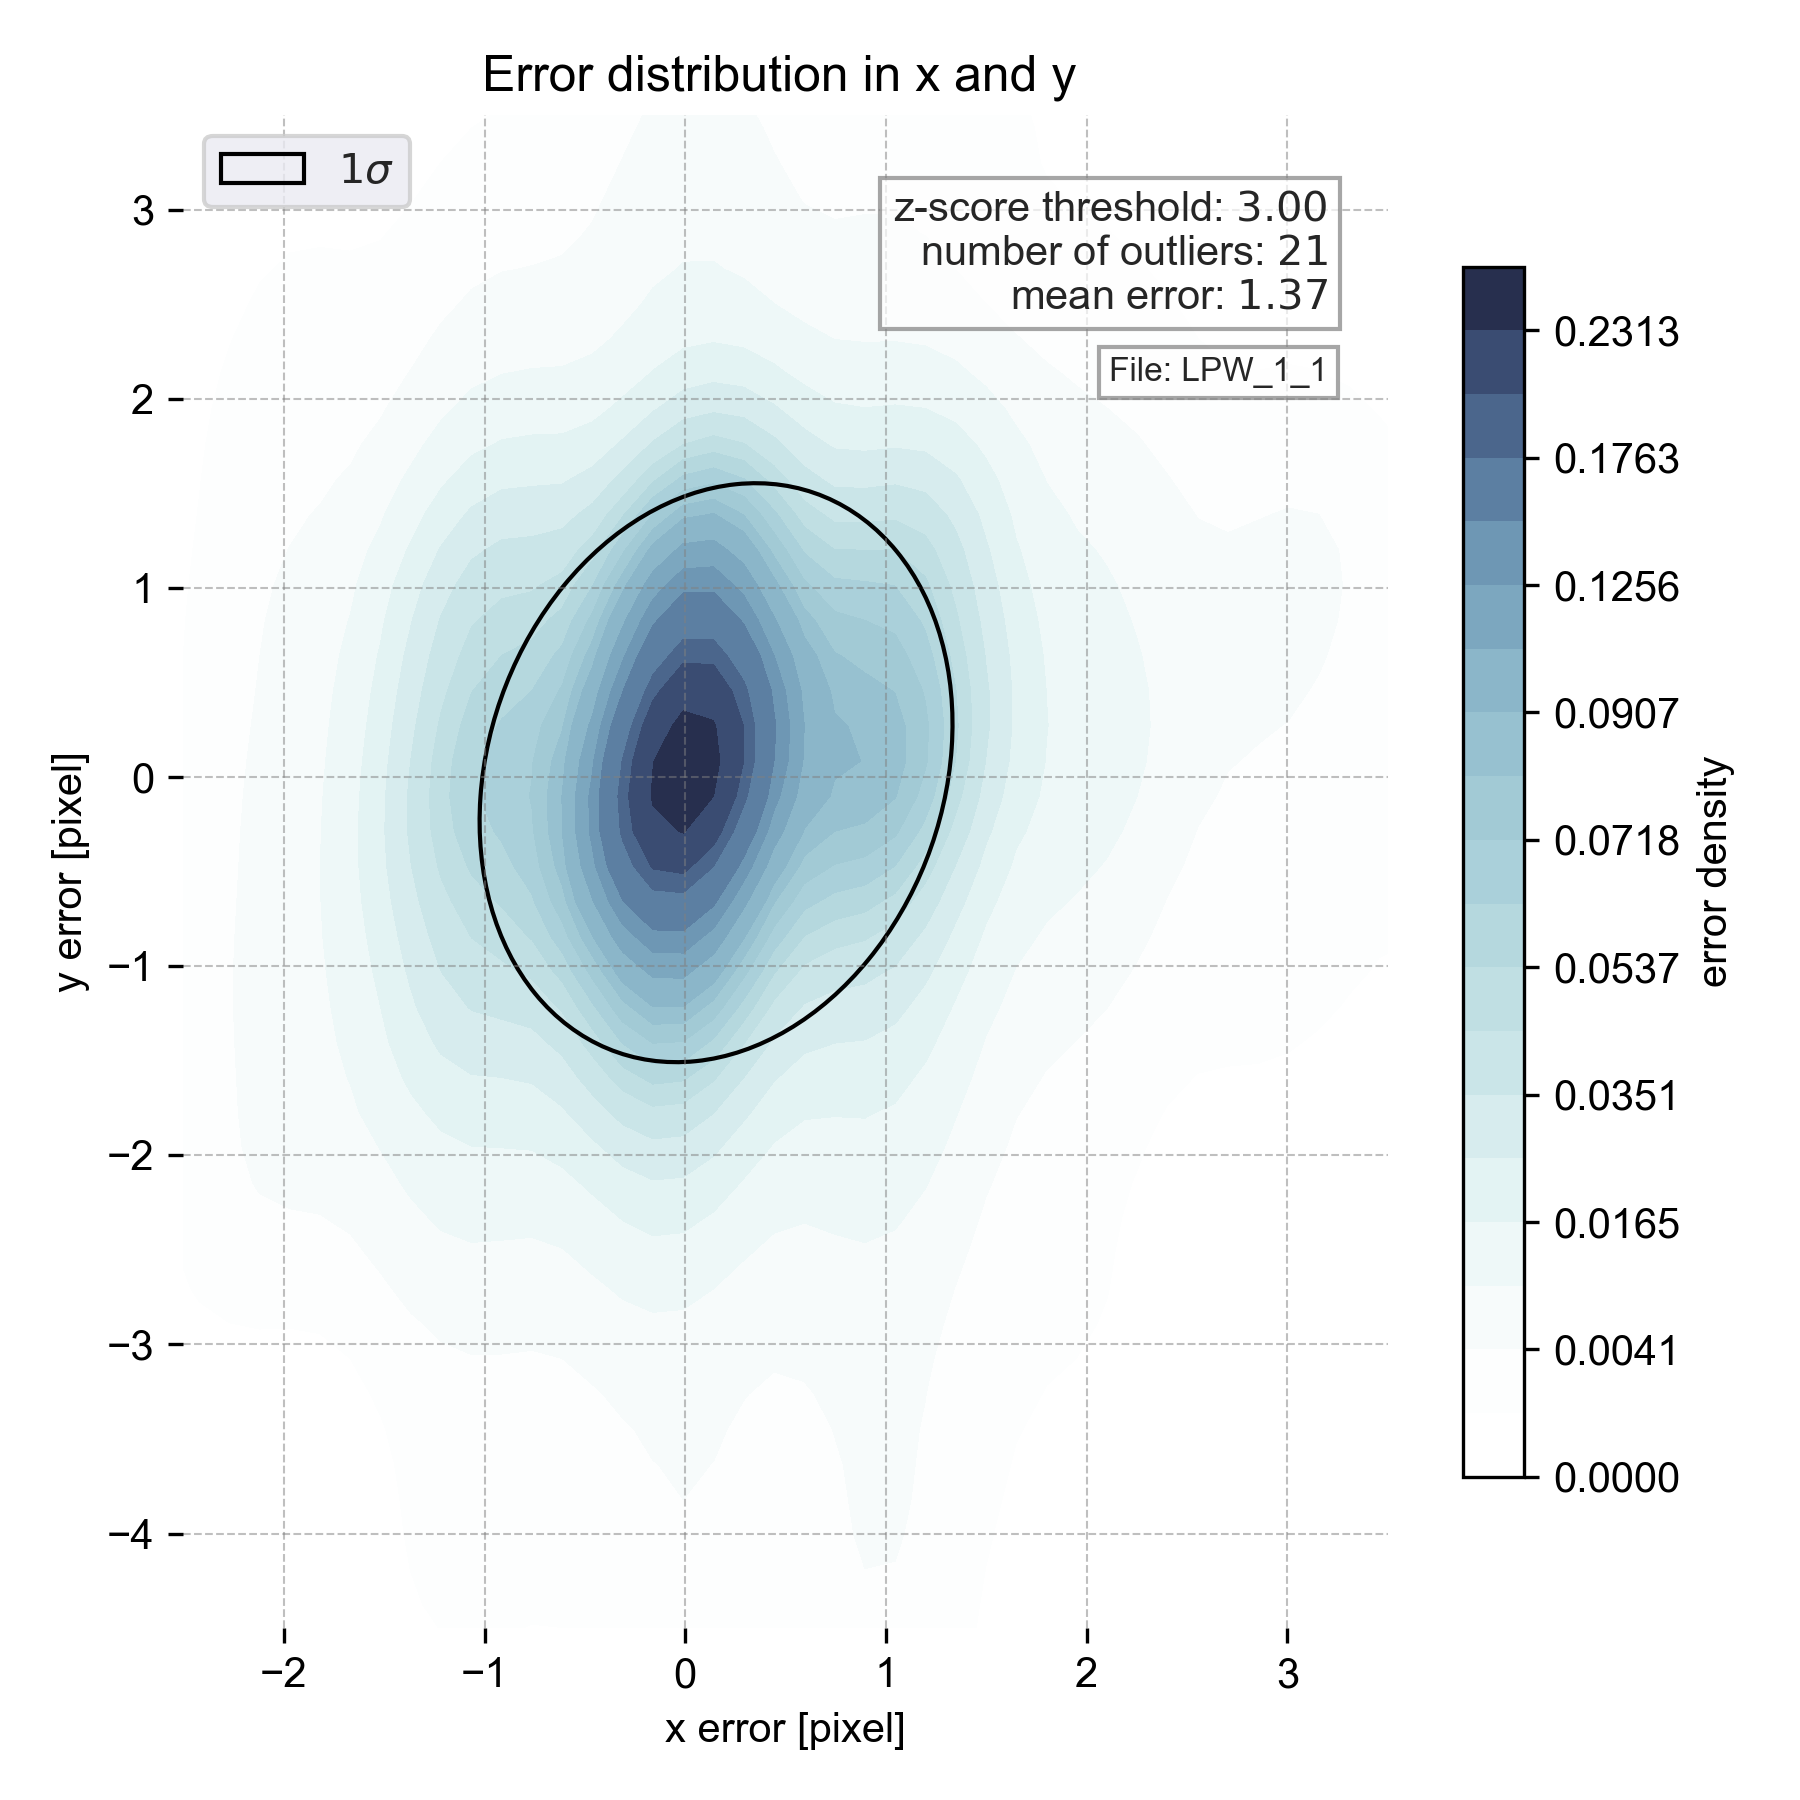
\includegraphics[width=\textwidth]{plots/LPW_1_1pre.png}
        \caption{Full image size (640x480)}
        \label{fig:full_scale}
    \end{subfigure}
    \begin{subfigure}{0.49\textwidth}
        \centering
        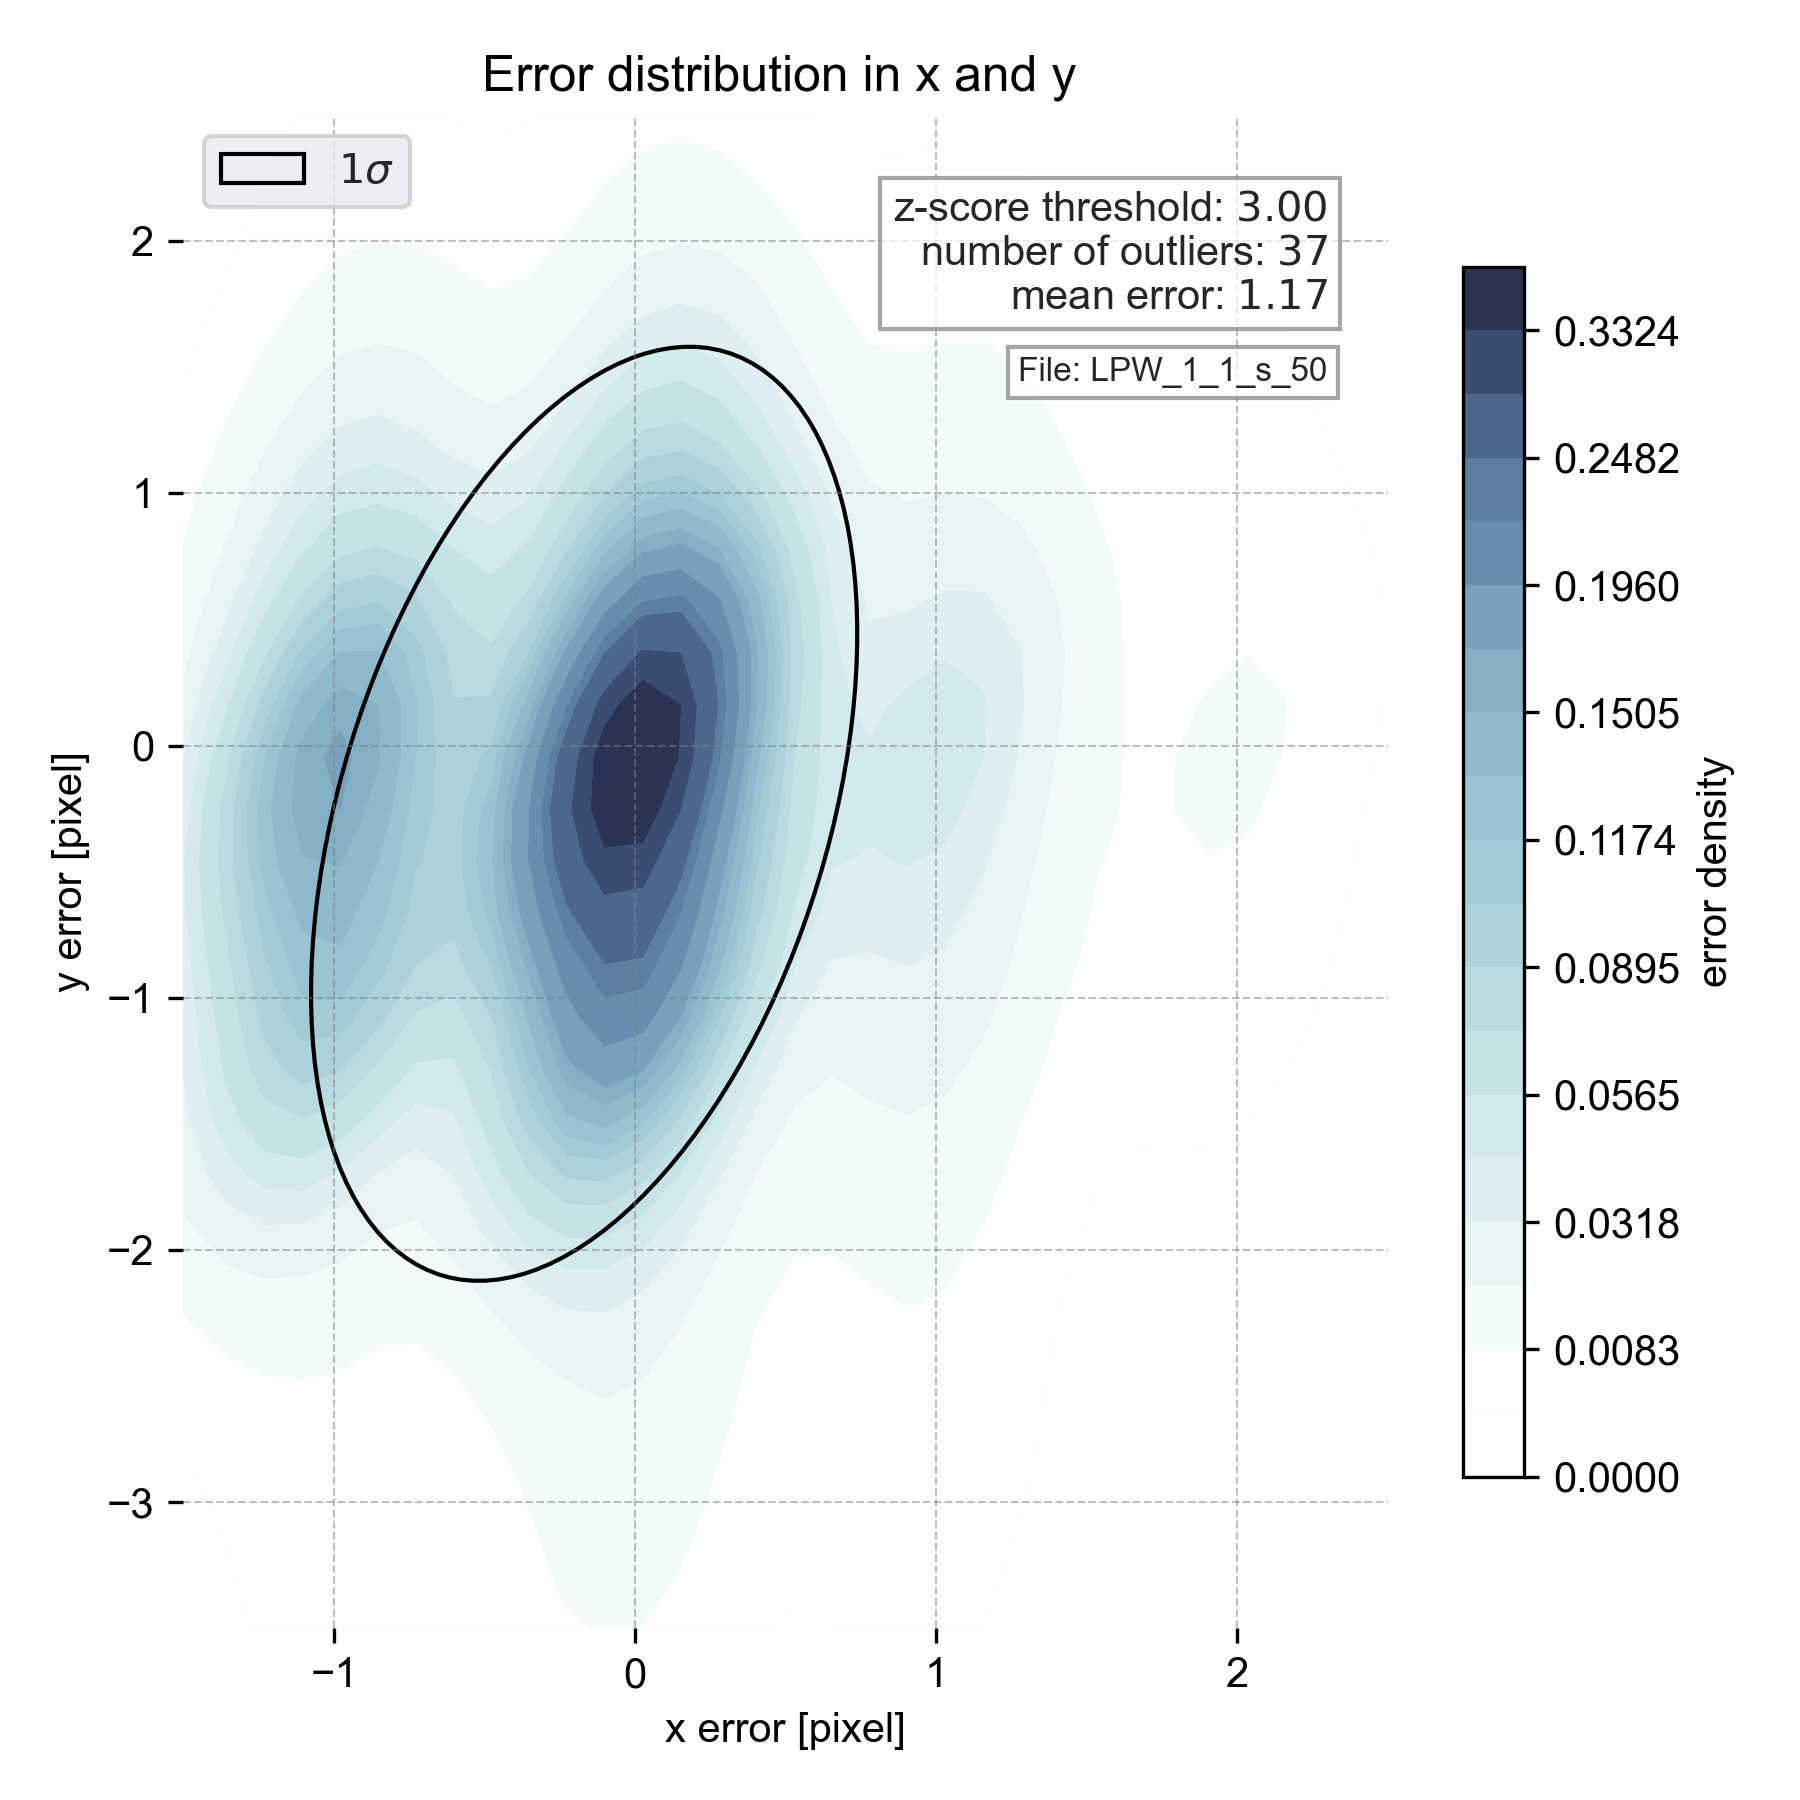
\includegraphics[width=\textwidth]{plots/LPW_1_1_s_50.png}
        \caption{Image size scaled by 0.5 (320x240)}
        \label{fig:halfscale}
    \end{subfigure}
    \caption{Comparing Error KDE plots of different image sizes}
    \label{fig:comp_e_size}
\end{figure}
Even though the mean error in figure \ref{fig:halfscale} seems to be lower, it needs to be considered that the number of outliers almost doubled when scaling the frames with a factor of 0.5 and the standard deviation also increases in the y direction but the mean error decreased. Nevertheless,  notable is that the Haar-like feature detected the pupil in every frame, no matter the scaling. This statement is not valid for all the LPW data set videos. By scaling the image, information is lost, including information about the pupil boundary. Important to note is that the parameters for the Haar-like feature and ACWE must be adapted to the scaling of the images. 
It is possible to get more accurate results by increasing the number of iterations of the RANSAC algorithm as well as $\lambda_1$ and $\lambda_2$ of the ACWE algorithm. This comes with the cost of speed, discussed in the next section. 
Another aspect of the accuracy is the fit of the ellipse itself. Even though the center has a considerably low error, the fit of the ellipse contour also tends to jump in a range of one or two pixels. This effect can also be seen when using scaled frames but does not necessarily increase with the scaling. The reason for this is the RANSAC algorithm that is used to fit the ellipse to the binary mask. This can be solved by using a higher number for iterations. The ACWE algorithm can also be a limiting factor because it stops at the pupil's outer boundary, which is not necessarily the same boundary as visually perceived.
\subsection{Speed}
The algorithm's speed is measured by the time it takes to process 2000 frames. The mean of the total time per frame is considered the speed of the algorithm. Currently, the algorithm runs at 1.2 fps, which equals 0.83  seconds per frame. This time was measured on full-scale images of the size 640x480. Decreasing the size significantly improves the speed and increases the ACWE algorithm's error, which is reflected in the ellipse fit. The parameters for the Haar-like feature and ACWE must be recalibrated for the new scaling. There is no general rule of thumb to scale the parameters. Also,  the algorithm's speed does not scale linearly with the size of the image.
\subsection{Robustness}
The algorithm's robustness is measured by the amount of outliers the algorithm produces. Calculating the z-score and setting the threshold to three times the standard deviation of the complete video makes it possible to filter outliers out and get a numerical value for robustness. In a full-scale video with reasonable noise, the haar-like feature can find a point in the pupil in every frame. The smaller the image gets, the less reliable the haar-like feature method becomes. However, even at a scaling of 0.5, the Haar-like feature detection performs at a success rate of 100 percent. The ACWE algorithm is the limiting factor for robustness. Because the RANSAC algorithm expects a certain amount of boundary points to fit the ellipse, the error will also be visible in the boundary approximation if the ACWE algorithm cannot extract the pupil boundary. The fewer border points are detected, the more iteration $N$ RANSAC needs to find the best fit. 
\subsection{Noise}

\section{Possible Improvements}
The algorithm has many parameters that can be tuned to improve the performance. The parameters that can greatly impact the performance are the parameters of ACWE introduced in section \ref{sus:acwe_ransac} and RANSAC parameters introduced in section\ref{sus:ransac}. The parameters are:
\begin{gather*}
    \text{ACWE: } \lambda_1, \lambda_2,\text{smoothing iteratios}, \text{Iterations}\\
    \text{RANSAC: } \alpha, \beta, \text{Iterations}, \text{Threshold}
\end{gather*}
Because the binary mask of the ACWE is used for the RANSAC, $\lambda_1$ and $\lambda_2$ are of great importance for the model's accuracy. If those parameters are chosen incorrectly, ACWE cannot extract the pupil area correctly. Therefore, the RANSAC will not be able to fit an accurate ellipse to the boundary of the pupil. $\lambda_1$ and $\lambda_2$ are sensible to the iris intensity. Darker colors need especially careful tuning. 

The number of Iterations is less critical for the ACWE because it has a stopping criteria when the contour converges, but it has to be chosen high enough so that the ACWE is not abruptly stopped before the contour has converged. If more smoothing iterations are chosen, the contour will grow and converge faster but will also be more inaccurate. So there is a tradeoff between speed and accuracy. 

The RANSAC algorithm is also sensitive to the choice of parameters. $\alpha$ and $\beta$ do not influence the speed but the accuracy. They are the weights for the importance of inliers or boundary points. The number of iterations affects the speed and accuracy. The more iterations are chosen, the more different ellipses are fitted, and the chance for a better fit is higher with the cost of speed.

The $threshold$ used to decide if a point is on the boundary or not also affects the accuracy. The threshold can impact the accuracy because the binary mask will not have a perfect elliptic boundary. Therefore, the RANSAC algorithm needs to have a certain threshold to decide if a point is on the boundary. 

More testing should be done to find the best values for the parameters. The proposed algorithm is currently unable to run in real-time and still needs some improvements and bug fixing to maximize the performance. The proposed algorithms should be implemented in C++ with more multithreading and parallelization to improve the performance further. 